\section{Macro and Controller}
\label{sec:impl}
\begin{figure}[!t]
\centering
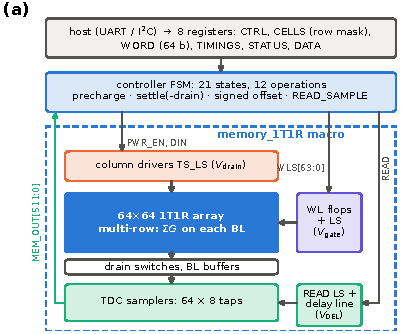
\includegraphics[height=1.4in]{macro_arch}\hfill
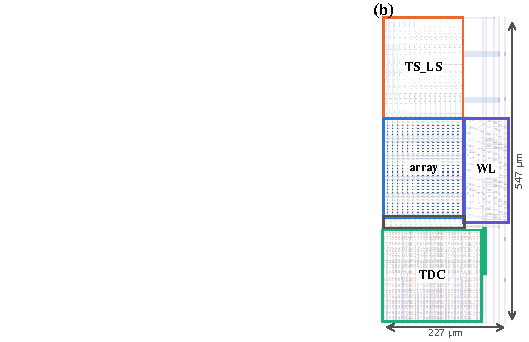
\includegraphics[height=1.4in]{macro_layout_crop}
\caption{(a) Macro and controller architecture. (b) Tape-out-ready layout, 226.5$\times$547.4\,\si{\micro\meter}.}
\label{fig:macro}
\end{figure}
The read path is implemented in a 64$\times$64 1T1R macro in the IHP SG13G2 130\,nm BiCMOS process, whose back-end HfAlO memristor (MEMRES) module~\cite{perez2017hfalo} provides the memory devices (Fig.~\ref{fig:macro}).
The array holds 4096 cells on a 2.26$\times$2.77\,\si{\micro\meter} pitch, each a high-voltage (HV) nMOS access transistor (W/L = 300/450\,nm) in series with a MEMRES device whose top electrode connects to the source line of its column (Fig.~\ref{fig:schematic}(a)).
Each column has a tri-state level-shifting driver supplied from $\Vd$ that drives SL or BL high for the writes and for the read precharge, and two global HV switches ground all source lines or all bit lines.
Each word line is driven through a pipeline flip-flop and a cross-coupled level shifter supplied from $\Vg$, so that an arbitrary 64-bit row mask written in one cycle opens any subset of rows in the next.
The delay line is shared by all 64 columns and supplied from the $\Vdel$ pad, and the 512 sampled bits return as the result of an access.

A 21-state finite-state machine (FSM) drives the macro with 12 operations, among them reads, SET, RESET, and mixed-polarity writes of a 64-bit word into the selected rows, a discharge-length test, and a sample capture that records sixteen codes along one discharge.
A read precharges for a programmable number of cycles, opens the row mask for a settle cycle with the source lines grounded, and then applies the drain step and READ with the signed offset of Section~\ref{sec:read}.
Eight 32-bit registers are written from a host over a serial link, and a host procedure searches $\Vg$, $\Vdel$, $\Vd$, the settle time, and the offset for the operating point that best separates the classes of each operation, as in Section~\ref{sec:eval}.
The macro is full custom and the controller is synthesized and placed around it; in an analog/mixed-signal simulation of the controller RTL against the macro netlist the sequenced reads return the codes of the stimulus-driven runs, and the design signs off at 100\,MHz in the slow corner with clean DRC, antenna, and LVS.
